

\chapter{Aplicação do Procedimento}

Os dados foram adquiridas via \textit{webscrapping} de um site nacional de aluguel de imóveis para 4 capitais brasileiras no dia 20 de Março de 2020, realizado pelo autor. Iremos estimar uma série de modelos com variadas configurações de hiperparametros, computar algumas métricas de sucesso e escolher os hiperparametros do modelo 'final' com base nisso. Essas métricas de sucesso serão computadas com dados omitidos no processo de treinamento, num processo chamado Validação Cruzada, e então aplicaremos o procedimento descrito no capítulo anterior.

\section{Otimização de Hiperparametros}

Não existe uma única maneira de estimar uma floresta aleatória. De fato, como machine learning é um campo que cresceu muito às margens da academia, em laboratórios da indústria, as convenções são informais e há pouco escrito em pedra. Optei por usar a implementação em \citeonline{ranger}, que usa como gatilho de geração de folhas uma amostra abaixo da mínima chegar no nodo e aleatoriza quantas variáveis explicativas são usadas em cada árvore. Uma alternativa de alta confiabilidade seria \citeonline{randomForest}. Para a otimização de hiperparâmetros, validação cruzada e avaliação dos modelos foi usada a plataforma \texttt{tidymodels} \cite{tidymodels}, implementada em linguagem R \cite{R}.

Decidida a implementação que irá realizar as computações, é preciso fazer uma escolha sobre os hiperparâmetros do modelo, no caso três: amostra mínima para criação de folha, número de árvores e número de variáveis a serem aleatoriamente escolhidas para cada árvore. Do ponto de vista do expectador desinteressado o problema é apenas:

\begin{align}
    \mathbf{x}^* = \underset{\mathbf{x}}{\text{arg max}} \,\,\phi(\mathbf{x}) 
\end{align}

E como seria fácil se soubéssemos exatamente o que é $\phi(\cdot)$, mas não sabemos. Uma primeira abordagem é tatear o suporte da função em busca da melhor combinação. Um método para isso é \textit{random search}, gerar algumas combinações de hiperparâmetros aleatórias, estimar um modelo em cada e escolher o de melhor performance, que definiremos em detalhes brevemente. O dual dessa abordagem é \textit{grid search} em que ao invés de gerar combinações aleatórias se cobre o espaço de hiperparâmetros de vetores com distância regular, gerando uma grade. 

Essas são ditas abordagens \textbf{caixa-preta livre de modelo} pois não fazem suposições sobre a forma funcional da função a ser maximizada ajustando os hiperparâmetros. Varremos o que acreditamos ser o seu domínio à força bruta. Existem alternativas. \citeonline{shahriari2015taking} é um tratamento amplo da principal, otimização bayesiana. Otimização de Hiperparâmetros é um campo grande. Um tratamento mais detalhado do estado da arte na área está disponível em \citeonline{feurer2019hyperparameter}.


\begin{figure}[H]
    \centering
    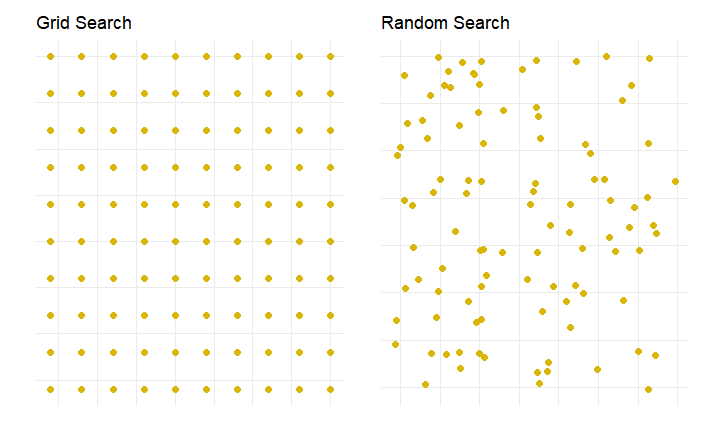
\includegraphics[scale = .75]{imagens/random_grid.png}
    \caption{Duas buscas de 100 modelos cada. Elaboração própria.}
\end{figure}

\section{Métricas de Qualidade}

Na seção anterior optamos por escolher hiperparâmetros de forma a maximizar alguma função que entendemos ser algo como a ''qualidade'' de um modelo. Precisamos agora definir como computa-la. Métricas de performance de modelo são sempre arbitrárias então a boa prática recomenda usar uma cesta delas. As opções para regressão são inúmeras. Serão avaliadas seis:

\begin{itemize}
    \item \textbf{Razão Performance-Interquatil (RPIQ)} \newline
    Definida como o desvio-padrão das previsões dividido pela amplitude interquartil da resposta. Mede principalmente a consistência do modelo, não a acurácia preditiva. Quanto mais próximo de 1, melhor. 
    
    \item \textbf{Coeficiente de Concordância de Correlação (CCC)} \newline
    Introduzido por \citeonline{lawrence1989concordance}, mede tanto consistência quanto acurácia. Calculada a partir da diferença entre a identidade e a reta de regressão dos valores preditos nos verdadeiros. Quanto mais próximo de 1, melhor.
    
    \item \textbf{Erro Médio Absoluto (MAE)} \newline
    A média das diferenças entre previsões e valores verdadeiros. Diretamente interpretável na unidade original da resposta. Indica acurácia. Menor é melhor, mas deve-se atentar à parcimônia.
    
    \item \textbf{Erro Médio Percentual (MPE)} \newline
    A média das diferenças entre previsões e valores verdadeiros ponderada pela média da resposta. Lida em unidades relativas. Indica acurácia. Menor é melhor, mas deve-se atentar à parcimônia.
    
    \item \textbf{Coeficiente de Determinação (R2)} \newline
    Calcula-se a soma dos quadrados dos desvios das previsões à média da resposta. Dividi-se esse valor pela soma dos quadrados dos desvios as observações originais à média da resposta. O resultado está entre $0$ e $1$ e pode ser interpretado como a fração da variância que o modelo consegue explicar. Mede principalmente consistência, não acurácia. Maior é melhor, mas deve-se atentar à parcimônia pois cresce monotonamente no número de variáveis explicativas.
    
    \item \textbf{Raiz do Erro Quadrático Médio (RMSE)} \newline
    O Erro Quadrático Médio é a média dos quadrados dos desvios das previsões em relação aos valores verdadeiros. A raiz dá a métrica. Mede principalmente acurácia, embora seja muito sensível a outliers. Menor é melhor.
    
\end{itemize}

Em um contexto de classificação precisamos de outras métricas. A título de exmeplo, algumas das mais comuns e fácil cálculo são:

\begin{itemize}
    \item \textbf{Sensitividade/ Recall} \newline
    Em classificação binária, a Sensitividade é a proporção dos casos positivos que são corretamente identificados.
    \item \textbf{Especificidade} \newline
    Em classificação binária, a Especificidade é a proporção dos casos negativos que são corretamente identificados.
    \item \textbf{Acurácia} \newline
    A fração de casos corretamente identificados. 
    \item \textbf{Precisão/ Valor Preditivo Positivo} \newline
    O número de verdadeiros positivos dividido pelo número de preditos positivos.
    \item \textbf{F1-Score} \newline
    Média harmônia da Precisão e da Sensitividade
    
\end{itemize}


\section{Validação Cruzada}

Para dar uma chance melhor a cada combinação podemos testa-la em amostras diferentes. Fazemos isso com validação $k$-cruzada. Dividimos a amostra em $k$ grupos aproximadamente iguais e para cada combinação de hiperparâmetros estimamos o modelo em $k-1$ combinações, excluindo um grupo de cada vez. Como medida de performance para cada combinação específica de hiperparâmetros usamos então a média das métricas de performance nas $k-1$ validações. 

Um pouco de sabedoria popular com florestas aleatórias sugere que o número de árvores não é um bom hiperparâmetro para se validar. Os ganhos de performance são pequenos, o custo computacional, no entanto, variante. Note que o custo de estimar uma floresta cresce linearmente, um para um, com o número de árvores. Validar $k$ combinações cada uma com $a*b$ árvores é $a$ vezes mais caro que validar $k$ combinações com $b$ árvores. 

Esse tempo de computação é melhor empregado procurando com uma grade fina melhores combinações de amostra única e número de variáveis por árvore. Árvores com menos variáveis tem menos variância, o que ajuda a diminuir a variância da floresta, e menor poder preditivo. Árvores com menor amostra mínima têm mais folhas, criando respostas mais finas, mas têm mais variância também. 


\begin{figure}[H]
    \centering
    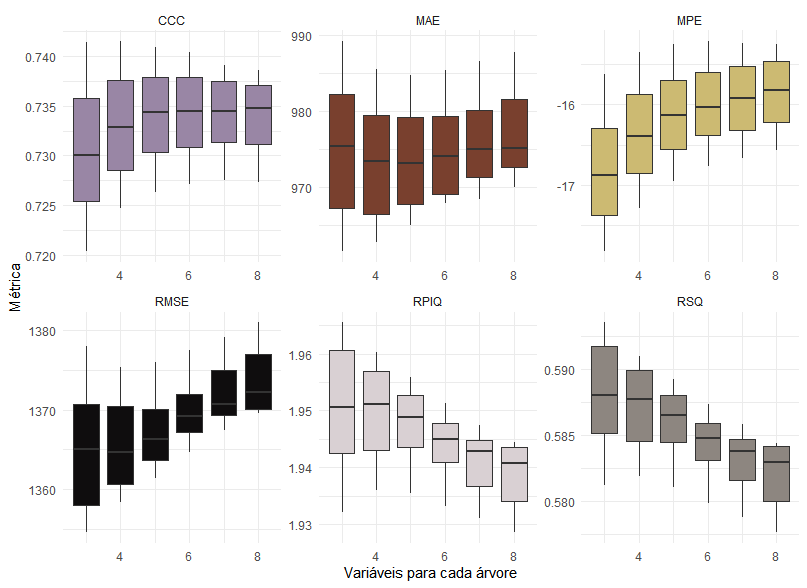
\includegraphics[scale = .72]{imagens/cross_v_mtry.png}
    \caption{Resumo de métricas de performance variando quantas variáveis alimentar para cada árvore. Elaboração própria.}
\end{figure}

Percorrendo o domínio de números de variáveis possíveis e mapeando o efeito em algumas métricas de performance vemos que nesse contexto esse hiperparâmetro não parece muito relevante, embora exista sim variação de performance. Ela, no entanto, não é consistente entre as métricas. Podemos, e devemos, verificar o que ocorre variando o tamanho de uma amostra que gatilha a geração de uma folha contendo uma regra de previsão/classificação. 


\begin{figure}[H]
    \centering
    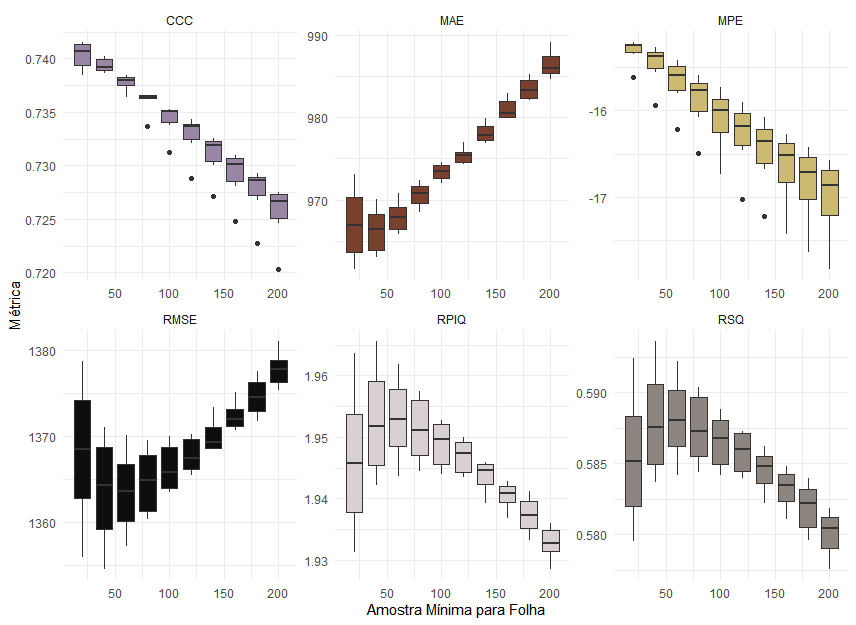
\includegraphics[scale = .70]{imagens/crossv_min.png}
    \caption{Resumo de métricas de performance variando a amostra mínima para criar uma folha. Elaboração própria.}
\end{figure}

Tabulando o melhor modelo de acordo com cada métrica temos:

\begin{table}[H]

\caption{\label{tab:tabela_metricas}Melhor modelo de acordo com cada métrica. Elaboração Própria.}
\centering
\begin{tabular}[t]{c|c|c}
\hline
Variáveis por Árvore & Amostra Mínima para Folha & metrica\\
\hline
3 & 20 & RPIQ\\
\hline
4 & 20 & CCC\\
\hline
3 & 20 & MAE\\
\hline
3 & 200 & MPE\\
\hline
3 & 20 & RSQ\\
\hline
3 & 20 & RMSE\\
\hline
\end{tabular}
\end{table}
\label{}{}



\section{Computação de Efeitos Marginais}
